\documentclass[11pt,a4paper,oneside]{article}

\newcommand{\mchname}{Mat\'{u}\v{s} Chochl\'{i}k}
\newcommand{\mchmail}{Matus.Chochlik@fri.uniza.sk}
\newcommand{\docnum}{Dnnnn=12-mmmm}
\newcommand{\docdate}{2012-03-08}

\usepackage[utf8]{inputenc}
\usepackage{url}
\usepackage{hyperref}
\usepackage{parskip}

\usepackage{listings}
\lstset{language=C++}

\usepackage{fancyhdr}
\setlength{\headheight}{14pt}
\pagestyle{fancyplain}
\lhead{\fancyplain{}{ISO/IEC JTC1 SC22 WG21 \docnum{} - Static reflection}}
\rhead{}
\rfoot{\fancyplain{}{\thepage}}
\cfoot{}

\setcounter{tocdepth}{2} 

\title{Static reflection}

\author{\mchname (\mchmail)}

\begin{document}

\begin{tabular}{r l}
Document number: & \docnum\\
Date: & \docdate\\
Project: & Programming Language C++, Library Working Group \\
Reply-to: & Mat\'{u}\v{s} Chochl\'{i}k (\href{mailto:\mchmail}{\mchmail})\\
\end{tabular}


\tableofcontents

\section{Introduction}

Reflection and reflective programming can be used
for a wide range of tasks such as implementation of serialization-like operations,
remote procedure calls, scripting, automated GUI-generation,
implementation of several software design patterns, etc.
C++ as one of the most prevalent programming languages 
lacks a standardized reflection facility.

In this paper we propose the addition of native support for
compile-time reflection to C++ and a library built
on top of the metadata provided by the compiler.

The basic static metadata provided by compile-time reflection
should be as complete as possible to be applicable in a wide
range of scenarios and allow to implement custom higher-level
static and dynamic reflection libraries and reflection-based
utilities.

The term \emph{reflection} refers to the ability of a computer program
to observe and possibly alter its own structure and/or its behavior.
This includes building new or altering the existing data structures,
doing changes to algorithms or changing the way the program code
is interpreted. Reflective programming is a particular kind
of \emph{metaprogramming}.

The advantage of using reflection is in the fact that everything
is implemented in a single programming language, and the human-written
code can be closely tied with the customizable reflection-based
code which is automatically generated by compiler metaprograms,
based on the metadata provided by reflection.

The solution proposed in this paper is based on the
\href{http://kifri.fri.uniza.sk/~chochlik/mirror-lib/html/}{\em Mirror}
reflection utilities~\cite{mirror-doc-cpp11} and on several years
of user experience with reflection-based metaprogramming.


\section{Motivation and Scope}

\subsection{Usefullness of reflection}

There is a wide range of computer programming tasks that involve
the execution of the same algorithm on a set of types defined by an
application or on instances of these types, accessing member variables,
calling free or member functions in an uniform
manner, converting data between the language's intrinsic representation and
external formats, etc., for the purpose of implementing the following:

\begin{itemize}

\item serialization or storing of persistent data in a
custom binary format or in XML, JSON, XDR, etc.,

\item (re-)construction of class instances
from external data representations (like those listed above),
from the data stored in a relational database, from data entered by
a user through a user interface or queried through a web service API,

\item automatic generation of a relational schema from the application
object model and object-relational mapping (ORM),

\item support for scripting 

\item support remote procedure calls (RPC) / remote method invocation (RMI),

\item inspection and manipulation of existing objects via a (graphic) user interface
or a web service,

\item visualization of objects or data and the relations between objects or
relations in the data,

\item automatic or semi-automatic implementation of certain software design patterns,

\item etc.

\end{itemize}

There are several aproaches to the implementation of such
functionality. The most straightforward and also usually the most
error-prone is manual implementation. Many of the tasks listed above
are inherently repetitive and basically require to process programming
language constructs (types, structures, containers, functions, constructors,
class member variables, enumerated values, etc.)
in a very uniform way that could be easily transformed into a meta-algorithm.

While it is acceptable (even if not very advantageous)
for example, for a design pattern implementation to be made by a human,
writing RPC/RMI-related code is a task much better suited for a computer.

This leads to the second, heavily used approach: preprocessing
and parsing of the program source text by a (usually very specfic) external
program (documentation generation tool, interface definition language compiler
for RPC/RMI, web service interface generator, a rapid application
development environment with a form designer, etc.) resulting in additional
program source code, which is then compiled into the final application binary.

This approach has several problems. First, it requires the external
tools which may not fit well into the build system or may not be portable
between platforms or be free; second, such tools are task-specific
and many of them allow only a limited, if any, customization of the output.

Another way to automate these tasks is to use reflection,
reflective programming, metaprogramming and generic programming as
explained below.

\subsection{Motivational examples}

This section describes some of the many possible uses of reflection
and reflective programming on concrete real-world examples.

\subsubsection{Factory generator}

As already said above, it is possible (at least partially) to automate 
the implementation of several established software design patterns.
This example shows how to implement a variant of the {\em Factory}
pattern.

By factory we mean here a class, which can create
instances of a {\em Product} type, but does not require that
the caller chooses the manner of the construction (in the programming
language) nor supplies the required arguments directly
in the C++ intrinsic data representation.

So instead of direct construction of a Product type,

\begin{lstlisting}
// get the values of arguments from the user
int arg1 = get_from_user<int>("Product arg1");
double arg2 = get_from_user<double>("Product arg2");
std::string arg3 = get_from_user<std::string>("Product arg3");
//
// call a constructor with these arguments
Product* pp = new Product(arg1, arg2, arg3);
// default construct a Product
Product p;
// copy construct a Product
Product cp = p;
\end{lstlisting}

which involves selection of a specific constructor, getting
the values of the required arguments and possibly converting 
them from an external representation and calling the selected
constructor with the arguments, 
factories pick or let the application user pick the Product's most
appropriate constructor, they gather the necessary parameters
in a generic way and use the selected constructor to create
an instance of the Product:

\begin{lstlisting}
// get data necessary for construction in xml
XMLNode xml_node_1 = get_xml_node(...);
XMLNode xml_node_2 = get_xml_node(...);

// make a factory for the product type
Factory<Product, XMLWalker> xml_factory;

// use the factory to create instances of Product
// from the external representation
Product p = xml_factory(xml_node_1);
Product* pp = xml_factory.new_(xml_node_2);
\end{lstlisting}

One of the interesting features of these factories is,
that they separate the caller (who just needs to get an instance
of the specified type) from the actual method of creation.

By using a factory, the constructor to be called can 
be automatically picked depending on the data available only at run-time
and not be chosen by the programmer (at least not directly
as in the code above). Factory can match
the constructor to best fit the data available in the external
representation (XML or JSON fragment, dataset resulting from a
RDBS query, etc.)

Even more interesting is, that such factories can be
implemented semi-automatically with the help of reflection.

Every factory is a composition of two distinct (an nearly orthogonal)
parts:

\begin{itemize}
\item{Product-type-dependent}: includes the enumeration of Product's
constructors, enumeration of their parameters, information about
the context in which a constructor is called, etc. This part is based
on reflection and independent on the representation of the input data.

\item{Data representation-dependent}: includes the scanning of the
available input data, conversion into C++ intrinsic data representation,
and the selection of the best constructor. This part is user-defined
and specifies how the input data is gathered and converted into the
C++ representation.
\end{itemize}

\begin{figure}[!th]
\centering
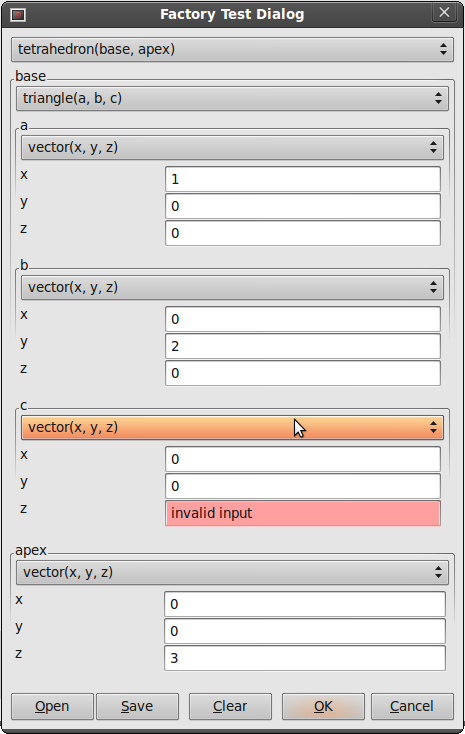
\includegraphics[width=.5\textwidth]{fact_tetrahedron.png}
\caption{Example of a GUI created by a factory generated by
the Mirror's factory generator.}
\label{fig:fact-tetrahedron}
\end{figure}

These two parts are then tied together into the factory class. Based
on the input-data related components, the factory can include a script parser
or XML document tree walker or code dynamically generating a GUI
for the input of the necessary values and the selection of the preferred
constructor. Figure \ref{fig:fact-tetrahedron} shows such a GUI created
by factory automatically generated by the Mirror's {\em factory generator}
utility for a tetrahedron class with the following definition:

\begin{lstlisting}
struct vector
{
        double x,y,z;

        vector(double _x, double _y, double _z)
         : x(_x)
         , y(_y)
         , z(_z)
        { }

        vector(double _w)
         : x(_w)
         , y(_w)
         , z(_w)
        { }

        vector(void)
         : x(0.0)
         , y(0.0)
         , z(0.0)
        { }

        /* other members */
};

struct triangle
{
        vector a, b, c;

        triangle(
                const vector& _a,
                const vector& _b,
                const vector& _c
        ): a(_a)
         , b(_b)
         , c(_c)
        { }

        triangle(void){ }

        /* other members */
};

struct tetrahedron
{
        triangle base;
        vector apex;

        tetrahedron(const triangle& _base, const vector& _apex)
         : base(_base)
         , apex(_apex)
        { }

        tetrahedron(
                const vector& a,
                const vector& b,
                const vector& c,
                const vector& d
        ): base(a, b, c)
         , apex(d)
        { }

        /* other members */
};

\end{lstlisting}


\section{Impact On the Standard}

\section{Design Decisions}

\subsection{Desired features} 

The proposed reflection facility is designed with the following
goals in mind:

\begin{itemize}
\item {\em Reusability}: The provided metadata should be reusable
in many situations and for many different purposes, not only
the obvious ones. This is closely related to {\em completeness} (below).

\item {\em Flexibility}: The basic reflection and the libraries
built on top of it should be designed
in a way that they are eventually usable during both compile-time
and run-time and under various paradigms (object-oriented, functional, etc.),
depending on the application needs.

\item {\em  Encapsulation}: The metadata should be accessible
through conceptually well-defined interfaces.

\item {\em  Stratification}: Reflection should be non-intrusive,
and the meta-level should be separated from the base-level language
constructs it reflects. Also, reflection should not be implemented
in a all-or-nothing manner. Things that are not needed, should not generally
be compiled-into the final application.

\item {\em  Ontological correspondence}: The meta-level facilities should
correspond to the ontology of the base-level C++ language constructs
which they reflect. This basically means that all existing language
features should be reflected and new ones should not be invented.
This rule may have some important exceptions like the reflection of
containers.

\item {\em  Completeness}: The proposed reflection facility should
provide as much useful metadata as possible, including various specifiers,
(like constness, storage-class, access, etc.), namespace members,
enumerated types, iteration of namespace members and much more.

\item {\em  Ease of use}: Although reflection-based metaprogramming
allows to implement very complicated things, simple things
should be kept simple.

\item {\em  Cooperation with other librares}: Reflection should be
usable with the existing introspection facilites (like \verb@type_traits@)
already provided by the standard library and with other libraries.
\end{itemize}

\subsection{Layered approach and extensibility}

The purpose of this section is to show that a {\em static} $\to$ {\em dynamic}
and {\em basic} $\to$ {\em complex} approach in designing reflection
can accomodate a wide variety of programming styles and is arguably
the "best" one. It does not propose to add all layers described
below into the standard library.

The Mirror reflection utilities \cite{mirror-doc-cpp11} on which this
proposal is based, implements several distinct components which
are stacked on top of each other. From the low-level metadata, through
a functional-style compile-time interface to a completely dynamic
object-oriented run-time layer (all described in greater detail below).

\subsubsection{Basic metaobjects}
The very basic metadata, which are in Mirror
provided (registered) by the user (or an automated command-line tool) via a set
of preprocessor macros. This approach is both inconvenient and error-prone
in many situations, but also has its advantages.

We propose that a standard compiler would make these basic metadata available
to the programmer through the basic metadata static interfaces. These would
serve as the basis for other (standard and non-standard) higher-level
reflection libraries and utilities.

In the Mirror utilities the basic metadata are not used directly by the
applications.

\subsubsection{Mirror}

A compile-time functional-style reflective programming library,
which is based directly on the basic metadata and is suitable for generic programming,
similar to the standard \verb@type_traits@ library.
It provides a more user-friendly and rich interface than the basic-metaobjects.

Mirror also provides a set of metaprogramming utilities which allow
to write compile-time meta-programs, which can generate efficient
and optimized program code using only those metadata that are required.

The following code shows several (rather simple) examples of usage
and the functional style of the algorithms based on metadata provided by Mirror.

The first example gets all types (registered) in the global scope,
applies some \verb@type_traits@ modifiers like \verb@std::add_pointer@
\verb@std::add_const@ and for each of such modified types calls a functor
that prints the names of the individual types to the standard output:

\begin{lstlisting}
struct name_printer
{
    template <typename MetaNamedObject>
    void operator()(MetaNamedObject mo) const
    {
        std::cout << mo.base_name() << std::endl;
    }
};

int main(void)
{
  using namespace mirror;
  // this function calls the name_printer functor passed
  // as the function argument on each element in the 
  // range that is passed as the template argument
  mp::for_each<
    // this template transforms the elements in the range
    // passed as the first argument by the unary template
    // passed as the second argument
    mp::transform<
      // this template filters out only those metaobjects
      // that satisfy the predicate passed as the second
      // argument from the range of metaobjects passed
      // as the first argument
      mp::only_if<
        // this template "returns" a range of metaobjects
        // reflecting the members of the namespace
        // (or other scope) that is passed as argument
        members<
          // this macro expands into a class
          // conforming to the Mirror's MetaNamespace
          // concept and provides metadata describing
          // the global scope namespace.
          // in the proposed solution for standard C++
          // this would be relaced by a special stdlib
          // function or by an operator.
          MIRRORED_GLOBAL_SCOPE()
        >,
        // this is a lambda function testing if its first
        // argument falls to the MetaType category
        mp::is_a<
          mp::arg<1>,
          meta_type_tag
        >
      >,
      // this is a unary lambda function that modifies the
      // type passed as its argument by the add_pointer
      // and add_const type traits
      apply_modifier<
        mp::arg<1>,
        mp::protect<
          std::add_pointer<
            std::add_const<
              mp::arg<1>
            >
          >
        >
      >
    >
  >(name_printer());
  std::cout << std::endl;
  return 0;
}

\end{lstlisting}


\subsection{Compile-time vs. Run-time reflection}

Run-time, dynamic reflection facilities may seem more readily
usable, but with the increasing popularity of compile-time metaprogramming,
the need for compile-time introspection (already taken care of
by \verb@type_traits@) and reflection also increases.

Also, if compile-time reflection is well supported it is relatively
easy to implement run-time or even dynamically loadable reflection
on top of it. The oposite is not true: One cannot use run-time metaobjects
or the value returned by their member functions as template parameters
or compile-time constants.

From the performance point of view, algorithms based on static
meta-data offer much more possibilities for the compiler to do
optimizations.

Thus, taking shortcuts directly to run-time reflection, without
compile-time support has obvious drawbacks.


\section{Technical Specifications}

We propose that the basic metadata describing a program written
in C++ should be made available through a set of {\em anonymous} classes
defined by the compiler. These classes should describe various program
constructs like, namespaces, types, typedefs, classes, their member variables
(member data), member functions, inheritance, templates, template parameters,
enumerated values, etc.

The compiler should generate metadata for the program constructs defined
in the currently processed translation unit. Indexed sets of metaobjects,
like scope members, parameters of a function, etc. should be listed
in the order of appearance in the processed source code.

Since we want the metadata to be available at compile-time,
different base-level constructs should be reflected by
{\em "statically" different} metaobjects and thus by {\em different} types.
For example a metaobject reflecting the global scope namespace should
be a different {\em type} than a metaobject reflecting the \verb@std@
namespace, a metaobject reflecting the \verb@int@ type should
have a different type then a metaobject reflecting the \verb@double@
type, a metaobject reflecting \verb@::foo(int)@ function should
have a different type than a metaobject reflecting \verb@::foo(double)@,
function, etc.

In a manner of speaking these special types (metaobjects) should become
"instances" of the meta-level concepts (static interfaces which
should not exist as concrete types, but rather only at the
"specification-level" similar for example to the iterator concepts).
This section describes a set of metaobject concepts,
their interfaces, tag types for metaobject classification and
functions (or operators) providing access to the metaobjects.

\subsection{Metaobject Concepts}

This section describes the requirements that various metaobjects
need to satisfy in order to be considered models of the individual
concepts.

\subsubsection{Categorization and Traits}

In order to provide means for distinguishing between regular types
and metaobjects the \verb@is_metaobject@ trait should be added
and should "return" \verb@true_type@ for metaobjects (types defined
by the compiler providing metadata) and \verb@false_type@
for non-metaobjects (native or user defined types).

The \verb@metaobject_traits@ structure should be defined to provide
categorization and additional information about the interface of metaobjects.

\begin{lstlisting}
template <typename Metaobject>
struct metaobject_traits
{
	typedef typename Metaobject::category category;

	typedef Bool has_name;

	typedef Bool has_scope;

	typedef Bool has_members;

	typedef Bool has_template;
};
\end{lstlisting}

The meaning of the individual trait typedefs is following:

\begin{itemize}
\item{\verb@category@} Is one of the following types and specifies the category
of the metaobject:
	\begin{itemize}
		\item{\verb@specifier_tag@} indicates a {\metaobject Specifier}.
		\item{\verb@namespace_tag@} indicates a {\metaobject Namespace}.
		\item{\verb@type_tag@} indicates a {\metaobject Type}.
		\item{\verb@typedef_tag@} indicates a {\metaobject Typedef}.
		\item{\verb@class_tag@} indicates a {\metaobject Class}.
		\item{\verb@function_tag@} indicates a {\metaobject Function}.
		\item{\verb@constructor_tag@} indicates a {\metaobject Constructor}.
		\item{\verb@operator_tag@} indicates an {\metaobject Operator}.
		\item{\verb@overloaded_function_tag@} indicates an {\metaobject OverloadedFunction}.
		\item{\verb@template_tag@} indicates a {\metaobject Template}.
		\item{\verb@enum_tag@} indicates an {\metaobject Enum}.
		\item{\verb@enum_value_tag@} indicates an {\metaobject EnumValue}.
		\item{\verb@inheritance_tag@} indicates an {\metaobject Inheritance}.
		\item{\verb@variable_tag@} indicates a {\metaobject Variable}.
		\item{\verb@parameter_tag@} indicates a {\metaobject Parameter}.
	\end{itemize}

\item{\verb@has_name@} indicates that the reflected object is {\metaobject Named}.
\item{\verb@has_scope@} indicates that the reflected object is {\metaobject Scoped}.
\item{\verb@has_members@} indicates that the reflected object is a {\metaobject Scope}.
\item{\verb@has_template@} indicates that the reflected object is {\metaobject Templated}.
\end{itemize}

\subsubsection{Metaobject}

{\metaobject Metaobject} is a stateless anonymous \verb@struct@ that provides
metadata reflecting certain program constructs and has the following properties:

\begin{itemize}
\item For every {\metaobject Metaobject} the \verb@is_metaobject@ trait returns \verb@true_type@.
\item For every {\metaobject Metaobject} the \verb@metaobject_traits@ structure is defined.
\item For every {\metaobject Metaobject} the {\verb@typedef Metaobject::category@} is defined
and has the same meaning as \verb@metaobject_category<Metaobject>::category@.
\end{itemize}

The exact type of a specific {\metaobject Metaobject} reflecting a specific
program feature is not defined by the standard, instances of metaobjects
should be always declared through the \verb@auto@ type specifier.

All instances of a specific {\metaobject Metaobject} should be equal to
the programmer and no internal context should be visible on the outside.

\subsubsection{Specifier}

{\metaobject Specifier} is a {\metaobject Metaobject}, which reflects specifiers like
\verb@const@, \verb@volatile@, \verb@private@,
\verb@protected@, \verb@public@, \verb@virtual@, etc. and has the following
interface:

\begin{itemize}

\item{\verb@static const char* keyword(void);@} returns the keyword
of the reflected specifier. If \verb@category@ is \verb@spec_none_tag@
then \verb@keyword@ returns "" (an empty c-string).

\item{\verb@typedef Category category;@} is defined as one of the following 
types:
	\begin{itemize}
		\item{\verb@spec_none_tag@} a category for missing specifiers,
		for example a non-const member function would have a \verb@spec_none_tag@
		constness specifier or a variable with automatic storage class
		would have a \verb@spec_none_tag@ storage class specifier, etc.

		\item{\verb@spec_extern_tag@} indicates \verb@extern@ storage class / linkage.
		\item{\verb@spec_static_tag@} indicates \verb@static@ storage class / linkage.
		\item{\verb@spec_mutable_tag@} indicates \verb@mutable@ storage class / linkage.
		\item{\verb@spec_register_tag@} indicates \verb@register@ storage class / linkage.
		\item{\verb@spec_thread_local_tag@} indicates \verb@thread_local@ storage class / linkage.

		\item{\verb@spec_const_tag@} indicates \verb@const@ member functions.

		\item{\verb@spec_virtual_tag@} indicates \verb@virtual@ inheritance or function linkage.

		\item{\verb@spec_private_tag@} indicates \verb@private@ member access.
		\item{\verb@spec_protected_tag@} indicates \verb@protected@ member access.
		\item{\verb@spec_public_tag@} indicates \verb@public@ member access.

		\item{\verb@spec_class_tag@} indicates the \verb@class@ elaborated type specifier.
		\item{\verb@spec_struct_tag@} indicates the \verb@struct@ elaborated type specifier.
		\item{\verb@spec_union_tag@} indicates the \verb@union@ elaborated type specifier.
		\item{\verb@spec_enum_tag@} indicates the \verb@enum@ elaborated type specifier.
	\end{itemize}
\end{itemize}

\subsubsection{Named}

{\metaobject Named} is a {\metaobject Metaobject} reflecting program constructs,
which have a name, like namespaces, types, functions, variables, etc. {\metaobject Named}
metaobjects have the following interface:

\begin{itemize}

	\item{\verb@static const char* base_name(void);@} returns the base name
	of the reflected construct, without the nested name specifier. For namespace
	\verb@std@ this function should return "std", for namespace \verb@foo::bar::baz@
	this function should return "baz", for the global scope this function
	should return "" (an empty c-string literal).\\For \verb@std::vector<int>::iterator@
	it should return "iterator". For derived and qualified types like \\
	\verb@volatile std::vector<const foo::bar::fubar*> * const *@ it should return
	"volatile vector$<$const fubar*$>$ * const *", etc.

	\item{\verb@static const char* full_name(void);@} returns the full name
	of the reflected construct, with the nested name specifier. For namespace
	\verb@std@ this function should return "std", for namespace \verb@foo::bar::baz@
	this function should return "foo::bar::baz", for the global scope this function
	should return "" (an empty c-string literal).\\For \verb@std::vector<int>::iterator@
	it should return "std::vector$<$int$>$::iterator". For derived and qualified types like\\
	\verb@volatile std::vector<const foo::bar::fubar*> * const *@ it should return
	"volatile std::vector$<$const foo::bar::fubar*$>$ * const *", etc.
\end{itemize}

The following is also true for {\metaobject Named} metaobjects.

\begin{itemize}
	\item \verb@metaobject_traits<Named>::has_name@ is defined as \verb@true_type@.
\end{itemize}

\subsubsection{Scoped}

{\metaobject Scoped} is a {\metaobject Metaobject} reflecting program constructs,
which are defined inside a scope (global scope, namespace, class, etc.). {\metaobject Scoped}
metaobjects have the following interface:

\begin{itemize}
	\item{\verb@typedef Scope scope;@} defined as a {\metaobject Scope} metaobject
	reflecting the scope of the scoped object.
\end{itemize}

The following is also true for {\metaobject Scoped} metaobjects.

\begin{itemize}
	\item \verb@metaobject_traits<Scoped>::has_scope@ is defined as \verb@true_type@.
\end{itemize}

\subsubsection{Scope}

{\metaobject Scope} is a {\metaobject Named} and {\metaobject Scoped} metaobject,
which reflects scopes like namespaces, classes, enums, etc. {\metaobject Scope}
has the following interface:

\begin{itemize}

	\item{\verb@typedef integral_constant<int,@ {\em number-of-scope-members}
	\verb@>@\\\verb@member_count;@} the total number of various members like types,
	namespace, functions, variables, etc. defined inside
	the scope reflected by a {\em Scope}.

	\item{\verb@static @{\em Scoped}\verb@ member(integral_constant<int, @{\em i}
	\verb@>);@} defined for $i \in \{0, 1, \dots, n-1\}$; {\em n = number-of-scope-members},
	each overload returns a different {\metaobject Scoped} metaobject reflecting the {\em i}-th member
	defined inside the scope reflected by a {\metaobject Scope}.
\end{itemize}

The following is also true for {\metaobject Scope} metaobjects.

\begin{itemize}
	\item \verb@metaobject_traits<Scope>::has_members@ is defined as \verb@true_type@.
\end{itemize}

\subsubsection{Namespace}

{\metaobject Namespace} is a {\metaobject Scope} for which the following is true:

\begin{itemize}
	\item \verb@metaobject_traits<Namespace>::category@ is defined as
	\verb@namespace_tag@.
\end{itemize}


\subsubsection{Type}

{\metaobject Type} is a {\metaobject Named} and {\metaobject Scoped} metaobject which
has the following interface:

\begin{itemize}
	\item{\verb@typedef @{\em original-type}\verb@ original_type;@} defined as the original type
	reflected by the {\metaobject Type}.
\end{itemize}

The following is also true for {\metaobject Type} metaobjects.

\begin{itemize}
	\item \verb@metaobject_traits<Type>::category@ is defined as \verb@type_tag@.
\end{itemize}

\subsubsection{Typedef}

\subsubsection{Class}

\subsubsection{Function}

\subsubsection{Constructor}

\subsubsection{Operator}

\subsubsection{OverloadedFunction}

\subsubsection{Template}

\subsubsection{Templated}

\subsubsection{Enum}

\subsubsection{EnumValue}

\subsubsection{Inheritance}

\subsubsection{Variable}

\subsubsection{Parameter}

\section{Acknowledgements}


\renewcommand\refname{\arabic{section}\hspace{1em}References}

\stepcounter{section}
\addcontentsline{toc}{section}{\refname}

\begin{thebibliography}{100}

\bibitem{mirror-doc-cpp11}
Mirror C++ reflection library documentation (C++11 version),
\url{http://kifri.fri.uniza.sk/~chochlik/mirror-lib/html/}.

\end{thebibliography}{100}



\end{document}
